\def\thelstlisting{}
\documentclass[american,english,runningheads]{llncs}

\usepackage[T1]{fontenc}
\usepackage[utf8]{inputenc}
\usepackage{url}
\usepackage[pdftex]{graphicx}
\usepackage[unicode=true,hidelinks]{hyperref}
\usepackage{times}
\usepackage{comment}
\setcounter{tocdepth}{2}

\clubpenalty=10000
\widowpenalty=10000
\tolerance=1000

\newcommand{\ie}{\emph{i.e.}}
\newcommand{\eg}{\emph{e.g.}}
\newcommand{\cf}{\emph{cf.~}}
\newcommand{\etal}{\emph{et al.~}}
\newcommand{\etc}{\emph{etc.}}
\newcommand{\aka}{\emph{a.k.a.}}

\newcommand{\noun}[1]{\textsc{#1}}

\newtheorem{mydef}{Definition}

\usepackage{hyperref}
\usepackage{listings}
%\usepackage[scaled]{luximono}


%\usepackage{natbib}

% ----- begin macros

\lstdefinelanguage{Scala}%
{morekeywords={abstract,%
  case,catch,char,class,%
  def,else,extends,final,for,%
  if,import,implicit,%
  match,module,%
  new,null,%
  object,override,%
  package,private,protected,public,%
  for,public,return,super,%
  this,throw,trait,try,type,%
  val,var,%
  with,%
  yield,%
  lazy%
  },%
  sensitive,%
  morecomment=[l]//,%
  morecomment=[s]{/*}{*/},%
  morestring=[b]",%
  morestring=[b]',%
  showstringspaces=false%
}[keywords,comments,strings]%

\lstdefinelanguage{JavaScript}%
{morekeywords={for, var, attributes, class, classend, do, else, empty, endif, endwhile, fail, function,
functionend, if, implements, in, inherit, inout, not, of, operations, out, return,
then, types, while, use},%
  sensitive,%
  morecomment=[l]//,%
  morecomment=[s]{/*}{*/},%
  morestring=[b]",%
  morestring=[b]',%
  showstringspaces=false%
}[keywords,comments,strings]%

\lstset{language=Scala,%
  mathescape=false,%
%  columns=[c]fixed,%
  aboveskip=\smallskipamount,
  belowskip=\smallskipamount,
%  basewidth={0.5em, 0.4em},%
  basicstyle=\ttfamily\small,%
  keywordstyle=\bfseries%\sffamily\bfseries,%
%  keywordstyle=\sffamily\bfseries,%
%  xleftmargin=0.5cm
}

\newcommand{\commentstyle}[1]{\slseries{#1}}
\newcommand{\keywordstyle}[1]{\bfseries{#1}}

\lstnewenvironment{slisting}{\lstset{language=Scala}}{}

\newcommand{\code}[1]{\lstinline[language=Scala,columns=fixed,basicstyle=\ttfamily\small]|#1|}

\def\changemargin#1#2{\list{}{\rightmargin#2\leftmargin#1}\item[]}
\let\endchangemargin=\endlist

%\setlength{\columnseprule}{0.25pt}

%\renewcommand{\note}[1]{$\spadesuit$ \textbf{#1} $\clubsuit$}


%\newcommand{\comment}[1]{}



\begin{document}

\setcounter{lstlisting}{0}
\renewcommand{\thelstlisting}{\arabic{lstlisting}}

\title{Statically typed Web programming}

\author{Julien \noun{Richard-Foy}\textsuperscript{\textasteriskcentered} \and Olivier \noun{Barais}\textsuperscript{\textasteriskcentered} \and
Tiark \noun{Rompf}\textsuperscript{\textdagger} \and Jean-Marc \noun{Jézéquel}\textsuperscript{\textasteriskcentered}}
\institute{\textsuperscript{\textasteriskcentered}IRISA, Université de Rennes 1, France: \texttt{\{first\}.\{last\}@irisa.fr}\\
\textsuperscript{\textdagger}EPFL, Lausanne, Switzerland: \texttt{\{first\}.\{last\}@epfl.ch}}

\authorrunning{Julien \noun{Richard-Foy} \etal{}}

\maketitle


\begin{abstract}
Rich Internet Applications involve more code on the client-side, dealing with DOM manipulation, event handling and
asynchronous calls to the server. Writing and maintaining large JavaScript code bases is challenging because this
language has several inadequacies (no static typing, no module system, verbose syntax, \etc{}). We investigate
further the definition of JavaScript as a Scala compiled embedded DSL using Lightweight Modular Staging. We define
safe and expressive abstractions for DOM manipulation, event handling and asynchronous programming that translate to
efficient JavaScript code using native APIs. We use both type-level information and staging to introduce high-level
abstractions with few or no overhead on the generated JavaScript code.
\end{abstract}

{\bf Keywords:} Web, programming languages, embedded DSL, type-level programming, staging, Scala

\section{Introduction}

The Web is an appealing platform on which to write applications (\aka{} Rich Internet Applications, RIA) because it
makes them easy to deploy on clients and allows large scale innovative collaborative
experiences~\cite{Farrell07_RIA,Mikkonen08_SpaghettiJs}. RIAs are characterized by partial updates of the user
interface (as opposed to refreshing the whole page with the classic hyperlink navigation), so a large part of the
client-side code listens to user interface events (such as mouse clicks), triggers the appropriate action
asynchronously on the server using AJAX~\cite{Garrett05_Ajax} and updates the application’s state and the DOM content
with a new DOM fragment computed from the response data~\cite{Farrell07_RIA,Busch09_StateOfArtRIA}.

Writing large Web applications is known to be
challenging~\cite{Mikkonen08_SpaghettiJs,Preciado05_RIAMethodologyNecessity}, mainly because of the heterogeneous
nature of the client-side and server-side environments~\cite{Echeverria09_RIA,Kuuskeri09_PartitioningClientServer}:
writing distributed code requires its parts to be consistent together and leads to duplication unless one uses the
same language in both sides, which, in the case of the Web, means using JavaScript to write the whole application.
However this language has several inadequacies making it hardly suitable for large code base (\eg{} no static typing,
no module system, verbose syntax, \etc). Some other in-browser execution environments give the opportunity to write
the client-side code in another language than JavaScript, \eg{} Java applets~\cite{Anuff96_JavaApplets}, Adobe
Flash~\cite{Curtis00_Flash} and Microsoft
Silverlight\footnote{\href{http://www.microsoft.com/silverlight/}{http://www.microsoft.com/silverlight/}}. However
these technologies have several drawbacks: they require an additional browser plugin to be installed (which may not
be available on all devices having a Web browser: for instance there is no way to execute Flash objects within an
Apple smart phone), the page content can't naturally be referenced by search engines, and the content is not
structured in URLs that users can bookmark or share.

An increasing number of initiatives attempt to allow developers to write the client-side code in a language different
than JavaScript but that can be compiled to JavaScript (\eg{} GWT~\cite{Chaganti07_GWT}, Dart~\cite{Griffith11_Dart},
TypeScript\footnote{\href{http://www.typescriptlang.org/}{http://www.typescriptlang.org/}}, Roy~\cite{McKenna_Roy}).
Some of these languages can also be compiled to another runtime environment usable on server-side (\eg{} GWT, Dart,
Kotlin\footnote{\href{http://kotlin.jetbrains.org/}{http://kotlin.jetbrains.org/}},
ClojureScript~\cite{McGranaghan11_ClojureScript}, Fay\footnote{\href{http://fay-lang.org/}{http://fay-lang.org/}},
Haxe~\cite{Cannasse08_HaXe} or Opa\footnote{\href{http://opalang.org/}{http://opalang.org/}}). These languages are
usually more suitable to write large applications either because they provide more constructs to build abstractions
(such as object orientation), or because they are statically typed, or because they add some useful concepts
that are missing in JavaScript (such as \emph{adhoc} polymorphism or namespaces). Moreover, their ability to compile
for both server and client sides usually allows developers to share some parts of code between server and client
sides for free. However this shared code is restricted to use exclusively language constructs: concepts provided by
external APIs can't be shared between server and client sides because the bindings with these environments are
different on the server and client sides.

In this paper we investigate further a path already introduced by Kossakowski \etal{}: defining JavaScript as a
compiled embedded DSL in Scala~\cite{Kossakowski12_JsDESL}. This approach is based on Lightweight Modular
Staging~\cite{Rompf12_LMSThesis}: a Scala program written using the embedded DSL evaluates to an intermediate
representation that can be further processed to perform domain specific optimizations and then to generate a
JavaScript program (for the client-side) and a Scala program (for the server-side). This approach has two main
advantages: (1) the embedding reduces the effort needed to define the language since we can reuse the Scala
infrastructure and tooling, and (2) staging gives more knowledge to the compiler about how a given abstraction
should be efficiently translated into the target environment. In other words any library-level abstraction can have
the efficiency of a language-level abstraction.

The previous work showed how to write client-side code in Scala using the JavaScript embedded DSL and how to share
code between server-side and client-side. The authors also showed that the code was safer and more convenient to
write thanks to Scala's static typing and class system. Finally, they showed how to \emph{un-invert} the control of
callback-based asynchronous APIs by using continuations but they did not address other concerns of RIAs development
such as user interface events handling, DOM creation and manipulation, and application’s state management.

This paper continues their work and presents safe and expressive DSL constructs for RIAs development. We increase the
expressivity of JavaScript native APIs with no runtime overhead and expose them through statically typed APIs. We
make asynchronous programming simpler by raising asynchronous computations to first-class citizen. We leverage the
Scala’s type system to bring type-directed language features such as \emph{adhoc} polymorphism and type coercion to
the client-side.

% This paper continues their work and presents and discusses the implementation of the following contributions:
% 
% \begin{itemize}
% 
% % JSDom, Forest
% \item We expose native JavaScript APIs for DOM manipulation and event handling as statically typed APIs while reducing their syntactic noise ;
% 
% % State monad, FutureOps, OptionOps
% \item We define a high-level abstraction to handle program's state changes and an abstraction turning asynchronous computations into first-class values. Then we show how to exploit staging to translate these abstractions into JavaScript with a minimal overhead ;
% 
% % NumericOps, Typeclasses
% \item We use Scala's advanced type-level constructs to elegantly express type coercion constraints on operands in arithmetic operations and to achieve \emph{adhoc} polymorphism with no overhead at all in the generated code ;
% 
% % Forest server-side, cross-browser incompatibilities
% \item Our code generation system is flexible enough to handle cross-browsers incompatibilities and, unlike other approaches, to allow the sharing of concepts between client-side and server-side even if these concepts are translated into code using external APIs.
% 
% \end{itemize}

The next section introduces a simple application example showing challenges of RIA development, section
\ref{solution} presents our DSL tackling these challenges, section \ref{validation} validates our solution and
compares it to related work and section \ref{discussion} concludes.

%\section{Web programming challenges?}

\section{Background and motivating example}
\label{problem}

To illustrate the challenges of writing a RIA and the need for a DSL for writing them, we introduce a simple “mind
mapping” application and show how the client-side code would be typically written in JavaScript.

\subsection{Example description}

In our application, a mind map is represented as a graph where ideas or concepts are represented by vertices, and the
relation between two ideas is represented by an edge. Users can visualize a mind map, zoom in and out and move it.
They can also add ideas and link them together. The figure \ref{mindmap} shows the visualization of a simple map
consisting of three ideas linked together, using our application.

\begin{figure}
 \caption{A simple mind map as visualized with our application}
 \centering
 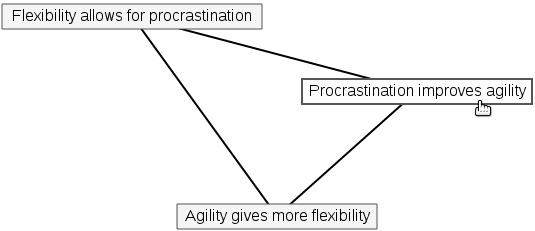
\includegraphics[width=8cm]{mindmap.png}
 \label{mindmap}
\end{figure}

\subsection{Implementation in JavaScript}

\subsubsection{Events handling}

RIAs distinguish themselves from classic Web pages by a higher degree of interactivity. In our example we want to let users zoom
in and out a map using their mouse wheel. To implement this feature we need to attach an event handler for the
\code{mousewheel} event on the DOM element containing the map. The following listing shows how to attach such an
event handler using the native JavaScript API:

\begin{lstlisting}[language=JavaScript,label=event-js,caption=Native JavaScript API to handle events]
mapElement.addEventListener("mousewheel", function (e) {
  scale = Math.round(scale + e.wheelDeltaY / 16);
  // ... update the user interface with the new scale
});
\end{lstlisting}

The event handler is simply a function taking the event data as a parameter. In the above example we use the
\code{wheelDeltaY} property of the event to update the scale of the map.

We think this code is fragile for two reasons. (1) The name of the event is passed as a string, so it is easy to
mispell it. (2) The callback passed as a second parameter takes a parameter \code{e} whose fields vary according to
the listened event but developers have no way to check that the fields they’re using are indeed defined on the event
they’re listening to. For instance, in our case we use the \code{wheelDeltaY} event field that is defined only on the
\code{mousewheel} event.

\subsubsection{Asynchronous programming}

Another characteristic of RIAs is that requests to the server are often performed asynchronously: instead of asking
the browser to reload the whole page, the JavaScript code has to perform a request and to process the response, when
available, to update a part of the user interface. The following listing shows how to send a request creating a
vertex on the server and to insert it to the user interface:

\begin{lstlisting}
var createVertex = function (text) {
  Ajax.post("/create", { content: text }, function (vertex) {
    addVertex(vertex);
  });
};
\end{lstlisting}

\code{Ajax.post} is a helper function that sends a HTTP request to the server and calls its last parameter
(that is a \emph{callback}) when the response data is available. The inverted control makes modularization harder to
achieve: in the above listing the function creating the vertex is also responsible of updating the user interface.
To relax this coupling the only option is to add a callback parameter to the \code{createVertex} function:

\begin{lstlisting}[language=JavaScript,label=async-js,caption=Callback-driven JavaScript APIs]
var createVertex = function (text, callback) {
  Ajax.get("/create", { content: text }, function (data) {
    callback(data);
  });
};

createVertex("Hello, World!", function (vertex) {
  addVertex(vertex);
});
\end{lstlisting}

However increasing the number of callbacks makes the code flow harder to follow and adds distance to the programmer's
initial intent.

Another issue with callback-driven programming arises when several dependent asynchronous computations are executed
sequentially. Consider for example the following listing performing three consecutive Ajax requests:

\begin{lstlisting}[language=JavaScript,label=async-callback-hell,caption=Sequential asynchronous calls]
Ajax.get(fooUrl(), function (foo) {
  Ajax.get(barUrl(foo), function (bar) {
    Ajax.get(bazUrl(bar), function (baz) {
      console.log(foo + bar + baz);
    });
    console.log("bar = " + bar)
  });
});
\end{lstlisting}

Notice that the code is getting deeper toward the right, this problem is often referred to as the
“callback-hell”~\cite{McKenna_Roy}. This code is also hard to reason about: when will the second \code{console.log}
statement be executed? Before or after \code{baz} has been fetched?

\subsubsection{DOM manipulation}
\label{forest}

Updating the user interface usually means replacing a part of the DOM with another DOM fragment computed from data
fetched by an AJAX request. This requires writing how to compute the new DOM fragment in JavaScript. For instance
the following listing shows how to build a DOM tree representing a vertex in the mind map:

\begin{lstlisting}[language=JavaScript,label=dom-api,caption=DOM fragment creation using the native API]
var vertexDom = function (v) {
  var root = document.createElement("g");
  root.setAttribute("class", "vertex");
  root.setAttribute("transform",
    "translate(" + v.x + "," + v.y + ")");
  var rect = document.createElement("rect");
  rect.setAttribute("width", v.width);
  rect.setAttribute("height", v.height);
  var text = document.createElement("text");
  text.setAttribute("width", v.width);
  text.setAttribute("height", v.height);
  text.appendChild(document.createTextNode(v.content));
  root.appendChild(rect);
  root.appendChild(text);
  return root
};
\end{lstlisting}

For instance the following call:
\begin{lstlisting}
vertexDom({
  x: 10, y: 10,
  width: 100, height: 60,
  content: "Hello, World!"
});
\end{lstlisting}
produces a DOM tree equivalent to the following HTML:
\begin{lstlisting}[language=HTML]
<g class=vertex transform="translate(10,10)">
    <rect width=100 height=60 />
    <text width=100 height=60>
        Hello, World!
    </text>
</g>
\end{lstlisting}

Not only the \code{vertexDom} function is very verbose, but it does not reflect the markup nested structure, making
it hard to read and reason about.

Another way to build a DOM tree is to build a String containing the desired markup and then to ask the browser to
parse it as HTML:

\begin{lstlisting}[language=JavaScript]
var vertexDom = function (v) {
  return '<g class=vertex ' +
             'transform="translate('+v.x+','+v.y+')">' +
           '<rect width='+v.width+' height='+v.height+' />' +
           '<text width='+v.width+' height='+v.height+'>' +
              v.content +
           '</text>' +
         '</g>'
};
\end{lstlisting}

The above code may be more readable, however this implementation is wrong: if we call it with a content containing
brackets (\eg{} \code{"<foo>"}) they won’t be escaped and will produce a \code{foo} tag nested in the \code{text} tag,
which is not the intended behavior. So, although this way reads slightly better it’s not less error prone.

By the way, unlike the previous points, markup generation is a task that often needs to be performed from both server
and client sides. From the server-side it produces HTML pages that search engines can crawl and from the client-side
it produces DOM fragments that can be used to update the user interface. So we want to share HTML fragments definition
between both server and client sides to get consistency in the rendering and to avoid duplication.

HTML template engines like Mustache\footnote{\href{http://mustache.github.com/}{http://mustache.github.com/}} or
Closure Templates\footnote{\href{https://developers.google.com/closure/templates/}{https://developers.google.com/closure/templates/}}
aim to make simpler the definition of DOM fragments by providing a convenient syntax to describe the HTML structure
and allowing the insertion of dynamic expressions in a safe way. Some template engines can be used on both
client-side and server-side, however none has a practical expression language (dynamic content can only be provided
as a map of key-value pairs and no operation can be done on values) or is statically typed.

\subsection{Assessment}
\label{assessment}

In the previous section we showed the three main tasks performed by the JavaScript code in RIAs: events handling,
asynchronous programming and DOM manipulation. We noticed the following issues:

\subsubsection{Lack of static checks}

Dynamic typing may give programmers more flexibility but can make it harder for little scripts to grow into mature
and robust code bases and to perform refactorings. For instance, in the case of RIAs, a mispell in an event name may
break the program behavior without getting a sensible error message.

\subsubsection{Code hard to reason about and to modularize}

Callback-driven APIs are very common in JavaScript but their inverted control makes the code flow hard to follow and
bothers modularization. Furthermore, native APIs are too verbose, making the code hard to read.

\subsubsection{Sharing type safe code between clients and servers is hard to achieve}

The lack of static checks is even harder to tackle in the case of code shared between client and server sides. If we
write the expression \code{xs.size == 0} in a template, how should it be translated to the client-side environment
(JavaScript) and to the server-side environment (\eg{} the Java Virtual Machine)? Several solutions are valid,
depending on the meaning of the expression: in JavaScript we could translate it as \code{xs.size === 0} or
\code{xs.length === 0} if \code{xs} refers to a collection (in JavaScript the property to get the size of a
collection is named \code{length}). We need to define a proper expression language and to define how it should be
translated for the client-side environment and the server-side environment, but such a task requires a high effort
and is hard to achieve in an extensible way (so users can still integrate their own data types in expressions instead
of being restricted to a set of supported types).

\section{DSL design and implementation}
\label{solution}

JavaScript libraries could address some of the challenges presented above, but addressing type safety and
asynchronous programming issues require language modifications (\eg{} to bring a type system and a sequencing
notation). Defining a language requires a high effort, especially to build development tools for the language so we
chose to define our language as a compiled embedded DSL in Scala\footnote{The code is available at
\href{http://github.com/js-scala}{http://github.com/js-scala}}.

\subsection{Introduction to Lightweight Modular Staging}
\label{intro-lms}

We use the Lightweight Modular Staging framework (LMS) to define our compiled embedded DSL. The main idea is that a
program written using a DSL is evaluated in two stages (or steps): the first stage builds an intermediate
representation of the program and the second stage transforms this intermediate representation into executable code
(figure \ref{lms-diagram}). The embedding lets us reuse the host language infrastructure (compiler, development
tools) and type system, and staging gives the opportunity to generate efficient code from expressive code by applying
domain specific optimizations.

\begin{figure}
  \centering
  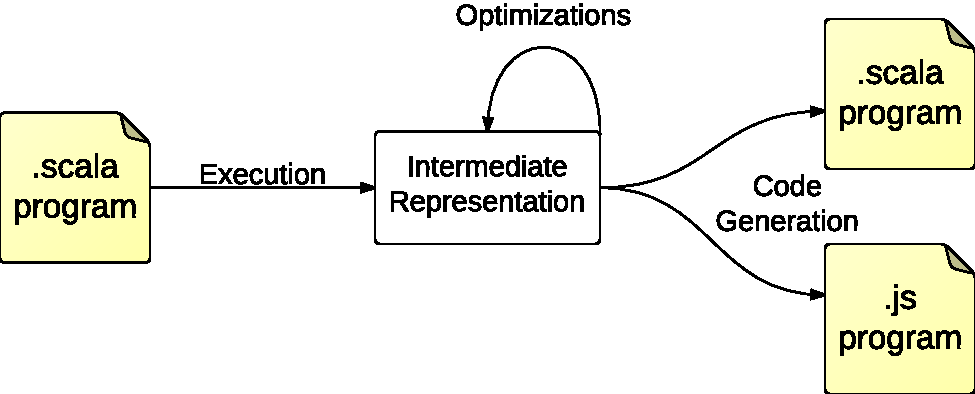
\includegraphics[width=7cm]{lms.pdf}
  \caption{Compilation of a program using LMS. An initial Scala program using embedded DSLs (on the left) evaluates
  to an intermediate representation from which the final program’s code is generated (on the right).}
  \label{lms-diagram}
\end{figure}

The bindings between stages are type-directed: a value of type \code{Rep[Int]} in the first stage will yield a value
of type \code{Int} in the second stage. If you consider the following code:
\begin{lstlisting}
val inc: Rep[Int] => Rep[Int] =
  x => x + 1
\end{lstlisting}
The function looks like
a regular Scala function excepted that its parameter type and its return type are wrapped in the \code{Rep[T]} type
constructor that denotes intermediate representations. The \code{+} operator has been defined on \code{Rep[Int]}
values and returns the intermediate representation of an addition. Finally, the \code{inc} function returns the
intermediate representation of a computation yielding the number following the value of the parameter \code{x}. You
can get a \code{T} value from a \code{Rep[T]} value by generating code from the intermediate representation and
compiling it:
\begin{lstlisting}
val compiledInc: Int => Int =
  compile(inc)
\end{lstlisting}
The \code{compile} function takes a staged program of type \code{Rep[A] => Rep[B]} and returns a final program of
type \code{A => B}.

The intermediate representation implementation is hidden for users but DSLs authors have to provide the corresponding
intermediate representation of each construct of their language. For that purpose, LMS comes with an extensible
intermediate representation implementation defining computations as a graph of statements. In the case of the
\code{inc} function, this graph contains a \code{Plus} node applied on a \code{Sym} node (the \code{x} parameter) and
a \code{Const} node (the literal value \code{1}).

Then, the code generation process consists in sorting this graph according to expressions dependencies and to emit
the code corresponding to each node. The listings \ref{codegen-js} and \ref{codegen-scala} show the JavaScript and
Scala generated code for the \code{inc} function:
\begin{multicols}{2}
\lstinputlisting[language=JavaScript, caption=JavaScript code generation, label=codegen-js]{inc.js}
\lstinputlisting[caption=Scala code generation, label=codegen-scala]{inc.scala}
\end{multicols}

Defining a DSL consists in three steps, each defining:

\begin{itemize}
\item The concrete syntax: an abstract API manipulating \code{Rep[_]} values~;
\item The intermediate representation: an implementation of the concrete syntax in terms of statement nodes~;
\item A code generator for the intermediate representation: a \emph{pretty-printer} for each DSL statement node.
\end{itemize}

The remaining of this section describe the design and the implementation of DSLs for Web programming using LMS.

\subsection{Events handling}

We want to bring safety to the events handling API so that developers can’t mispell an event name and can’t attempt
to read a property that is not defined on the type of the handled event. The difficulty comes from the fact that the
type of the event passed to the handler varies with the event name. For instance in the listing \ref{event-js}, the
handler processses \code{MouseWheelEvent} values because it listens to \code{mousewheel} events. Values of type
\code{MouseWheelEvent} have a property \code{wheelDeltaY} but that’s not the case of an event data of type
\code{KeyboardEvent}, for example.

A possible solution could be to define a distinct method for each event instead of the single \code{addEventListener}
method, so each method takes a handler with the according event type:

\begin{lstlisting}
window.onKeyUp { e: Rep[KeyboardEvent] =>
  println(e.key)
}
window.onMouseWheel { e: Rep[MouseWheelEvent] =>
  println(e.wheelDeltaY)
}
\end{lstlisting}

In the above listing, the \code{onKeyUp} method attaches an event handler for the \code{keyup} event that uses values
of type \code{KeyboardEvent}, and the \code{onMouseWheel} method does the same for \code{mousewheel} events that use
values of type \code{MouseWheelEvent}.

However, implementing this solution requires a high effort because we have to define as many methods as there are
events. We want to provide a single polymorphic method similar to the native API. To achieve that we need to encode
at the type-level the dependency relation between an event name and its corresponding event type. This dependency can
naturally and elegantly be encoded using dependent method types~\cite{Oliveira10_Typeclasses}:

\begin{lstlisting}
class EventDef {
  type Type
}

def on(ev: EventDef)(handler: Rep[ev.Type] => Rep[Unit]): Rep[Unit]
\end{lstlisting}

(We renamed \code{addEventListener} to \code{on}, for the sake of brevity). An \code{EventDef} value represents an
event that carries its corresponding event data type in its \code{Type} type member. The \code{on} method takes a
parameter \code{ev} of type \code{EventDef} and a \code{handler} parameter whose type refers to the \code{Type}
member of the \code{ev} parameter, so the type of the handler depends on the \code{ev} value. We can then define the
\code{keyup} and \code{mousewheel} events as follows:

\begin{lstlisting}
object KeyUp extends EventDef { type Type = KeyboardEvent }
object MouseWheel extends EventDef { type Type = MouseWheelEvent }
\end{lstlisting}

The following Scala listing is equivalent to the JavaScript listing \ref{event-js} and is completely type safe: if
the user misspells the event name or tries to use an undefined property on an event his program won’t compile.

\begin{lstlisting}
window.on(MouseWheel) { e =>
  scale = Math.round(scale + e.wheelDeltaY / 16)
}
\end{lstlisting}

\subsection{Asynchronous programming}

\begin{figure}
\centering
\begin{lstlisting}[caption=Asynchronous values are first class citizen,label=async-first-class]
def createVertex(text: Rep[String]): Rep[Future[Vertex]] =
  Ajax.post[Vertex]("/create", new Record { val content = text })

for (vertex <- createVertex("Hello, World!")) {
  addVertex(vertex)
}
\end{lstlisting}
\end{figure}

We propose a DSL that explicitly reflects the asynchronous nature of computations in their type and provides methods
turning them into first-class citizen. The DSL is monadic so we can solve the callback-hell problem thanks to the
Scala \code{for} notation.

For instance, listing \ref{async-first-class} shows how the listing \ref{async-js} can be
re-written with our DSL. The \code{createVertex} now returns an asynchronous value instead of taking a callback as
parameter. Then, the \code{for} expression allows us to use the vertex, when available, and to insert it on the user
interface. By making the \code{createVertex} function return an asynchronous value instead of taking a callback as
a parameter, the code is easier to modularize into loosely coupled parts.

\begin{figure}
\centering
\begin{lstlisting}[caption=No callback hell,label=async-no-callback]
for {
  foo <- Ajax.get(fooUrl())
  bar <- Ajax.get(barUrl(foo))
  _ <- future(println("bar = " + bar))
  baz <- Ajax.get(bazUrl(bar))
} println(foo + bar + baz)
\end{lstlisting}
\end{figure}

The listing \ref{async-no-callback} translates the “callback-hell” example (listing \ref{async-callback-hell}) using
our DSL. The \code{for} notation can intuitively be thought of as a sequencing notation: whenever the response of the
first Ajax request is available, the next statement will be executed, and so on. There is no nested callbacks and the
order of execution is directly reflected by the order of statements.

An asynchronous value of type \code{Rep[A]} is modelled by a value of type \code{Rep[Future[A]]}. Because Scala’s
\code{for} notation is just syntactic sugar for methods \code{foreach}, \code{map} and \code{flatMap}, we are
able to define our DSL by just defining these methods on \code{Rep[Future[A]]} values, with the following semantic:
\begin{itemize}
\item \code{foreach(f: Rep[A] => Rep[Unit]): Rep[Unit]}, eventually does something with the value when available~;
\item \code{map(f: Rep[A] => Rep[B]): Rep[Future[B]]}, eventually transforms the value when available~;
\item \code{flatMap(f: Rep[A] => Rep[Future[B]]): Rep[Future[B]]} eventually transforms the value when available~;
\end{itemize}

Asynchronous values can be transformed using the \code{map} and \code{flatMap} methods, turning them into first-class
citizen: functions can take as parameters and return asynchronous values.

\begin{figure}
\begin{multicols}{2}
\begin{lstlisting}[caption=Parallel computations in Scala,label=async-parallel-1]
val fooAsync = Ajax.get("/foo")
val barAsync = Ajax.get("/bar")
for {
  foo <- fooAsync
  bar <- barAsync
} println(foo + bar)
\end{lstlisting}
\vfill
\columnbreak
\begin{lstlisting}[language=JavaScript,caption=Generated JavaScript code,label=async-parallel-2]
var x1 = new Promise();
AjaxGet("/foo", x1);
var x2 = new Promise();
AjaxGet("/bar", x2);
x1.onComplete(function (foo) {
 x2.onComplete(function (bar) {
  var x3 = foo + bar;
  console.log(x3);
 });
});
\end{lstlisting}
\end{multicols}
\end{figure}

Listing \ref{async-parallel-1} and \ref{async-parallel-2} define two asynchronous computations running in parallel
and the generated JavaScript code (we renamed some identifiers for the sake of readability). The generated
\code{Promise} constructor code has been omitted, it creates an object holding a list of callbacks to call when the
asynchronous value is completed. The \code{AjaxGet} function code has also been omitted, it creates a
\code{XMLHttpRequest} object that sends an HTTP request and completes its promise parameter with the response, when
received.

% \begin{lstlisting}[caption=Concrete syntax of the asynchronous programming DSL]
% trait FutureOps { this: Base =>
% 
%   implicit def FutureOpsCls[A](f: Rep[Future[A]]): FutureOpsCls[A]
%   type FutureOpsCls[+A] <: FutureOpsBase[A]
% 
%   trait FutureOpsBase[+A] {
%     def map[B](f: Rep[A] => Rep[B]): Rep[Future[B]]
%     def flatMap[B](f: Rep[A] => Rep[Future[B]]): Rep[Future[B]]
%     def foreach(f: Rep[A] => Rep[Unit]): Rep[Unit]
%     def withFilter(f: Rep[A] => Rep[Boolean]): Rep[Future[A]]
%   }
% }
% \end{lstlisting}
% 
% The \code{FutureOps} module depends on the \code{Base} module defined by LMS. The \code{Base} module essentially defines the abstract type constructor \code{Rep[_]}. Values of type \code{Rep[Future[A]]} have no methods because the \code{Rep[_]} type is abstract and unbound, so we use an implicit conversion from \code{Rep[Future[A]]} to \code{FutureOpsCls[A]} to add methods to \code{Rep[Future[A]]} values. The type \code{FutureOpsCls[A]} is bound by the \code{FutureOpsBase[A]} trait that defines the signature of the methods added to \code{Rep[Future[A]]} values. Everything in the \code{FutureOps} module is abstract, these definitions only provide the vocabulary of the DSL.
% 
% The listing \ref{futureopsexp} shows the definition of the \code{FutureOpsExp} module that implements the \code{FutureOps} module and defines how statement nodes are built from the DSL constructs.
% 
% \begin{figure}
% \begin{lstlisting}[label=futureopsexp,caption=Definition of the intermediate representation of the asynchronous programming DSL]
% trait FutureOpsExp extends FutureOps { this: EffectExp =>
% 
%   implicit class FutureOpsCls[+A](a: Exp[Future[A]])
%       extends FutureOpsBase[A] {
%     def map[B](f: Exp[A] => Exp[B]) = {
%       val x = fresh[A]
%       val b = reifyEffects(f(x))
%       reflectEffect(FutureMap(a, x, b), summarizeEffects(b).star)
%     }
% 
%     // ... same for other methods (flatMap, foreach and withFilter)
%   }
%   
%   case class FutureMap[A, B](a: Exp[Future[A]], x: Sym[A], b: Block[B])
%       extends Def[Future[B]]
%   // ... same for other operations
% }
% \end{lstlisting}
% \end{figure}
% 
% The \code{FutureOpsExp} module depends on the \code{EffectExp} module that is a module refining the \code{Base} module, defining the type \code{Rep[A]} as \code{Exp[A]}, which is a base class defining intermediate representations as a graph of statements. The \code{EffectExp} module also provides tools to handle effectful statements. The implicit class \code{FutureOpsCls} implements both the abstract type and the implicit conversion of the same name defined in the \code{FutureOps} trait. Each method of the \code{FutureOpsCls} class is reified to a statement node, for instance the \code{map} method returns a \code{FutureMap} node containing a reference to the node on which the \code{map} operation is applied and the code block that was passed as a parameter to the \code{map} operation. We propagate the information about the effects performed by the statements in the code block by calling \code{reflectEffect} on our statement node.
% 
% The listing \ref{jsgenfutureops} shows the code of the JavaScript code generator for the DSL. The code generation process basically consists in traversing the graph of statement nodes and in emitting the code corresponding to each node. To implement a code generator for a given DSL we just need to say how to generate code for this DSL statement nodes.
% 
% \begin{figure}
%  \begin{lstlisting}[label=jsgenfutureops,caption=JavaScript code generator for the asynchronous programming DSL]
% trait JSGenFutureOps extends JSNestedCodegen {
%   val IR: EffectExp with FutureOpsExp
%   import IR._
% 
%   override def emitNode(sym: Sym[Any], rhs: Def[Any]) = rhs match {
%     case FutureMap(a, x, b) =>
%       emitValDef(sym, "new Promise()")
%       stream.println(quote(a) + ".onComplete(function (" + quote(x) + ") {")
%       emitBlock(b)
%       stream.println(quote(sym) + ".complete(" + quote(getBlockResult(b)) + ");")
%       stream.println("});")
%     // ... same for each node
%     case _ => super.emitNode(sym, rhs)
%   }
% }
%  \end{lstlisting}
% \end{figure}
% 
% The \code{JSGenFutureOps} code generator inherits from the \code{JSNestedCodegen} code generator that defines the building blocks of the JavaScript code generation. The main method is \code{emitNode}, it is called by LMS for each traversed node of the statement graph. In the listing we only showed the code generation for the \code{FutureMap} node: when the asynchronous value on which the \code{map} method has been applied is available, we apply the function passed to the \code{map} method on the value and complete a newly created asynchronous value with the result. The \code{Promise} constructor is provided by a JavaScript preamble and creates an asynchronous value with two methods: \code{onComplete}, registering a callback to be called when the value is available, and \code{complete}, fulfilling the promise with a value.


\subsection{DOM definition}

In this section we show how we can define, as an embedded DSL, with minimal effort, a template engine that is
statically typed, able to insert dynamic content in a safe way, that provides a powerful expression language,
requires no extra compilation step and that can be used on both client-side and server-side.

Because the template engine is defined as en embedded DSL, we can reuse Scala’s constructs:

\begin{itemize}
\item a function taking some parameters and returning a DOM fragment directly models a template taking parameters and
returning a DOM fragment~;
\item the type system typechecks template definitions and template calls~;
\item the Scala language itself is the expression language~;
\item compiling a template is the same as compiling user code.
\end{itemize}

So the only remaining work consists in defining the DSL vocabulary to define DOM nodes. We provide a \code{tag}
function to define a tag and a \code{text} function to define a text node. The following listing uses our DSL and
generates a code equivalent to the listing \ref{dom-api}:

\begin{lstlisting}[label=forest-hello,caption=DOM definition DSL]
def vertexDom(v: Rep[Vertex]) =
    tag("g", "class"->"vertex",
             "transform"->("translate("+v.x+","+v.y+")"))(
        tag("rect", "width"->v.width, "height"->v.height)(),
        tag("text", "width"->v.width, "height"->v.height)(
            text(v.content)
        )
    )
\end{lstlisting}

The readability has been highly improved: nesting tags is just like nesting code blocks, HTML entities are
automatically escaped in text nodes, developers have the full computational power of Scala to inject dynamic data and
DOM fragments definitions are written using functions so they compose just as functions compose. These benefits come
with no performance loss because the DSL generates code building DOM fragments by using the native JavaScript API.

\subsubsection{Reuse the DOM definition DSL on server-side}

Our DSL is equivalent to a template engine with Scala as the expression language. Making it usable on both server and
client sides is surprisingly as simple as defining another code generator for the DSL, producing Scala code.

For instance, the template written in the listing \ref{forest-hello} produces the following Scala code usable on
server-side (the generated code for client-side is roughly equivalent to the listing \ref{dom-api}):

\begin{lstlisting}
def vertexDom(v: Vertex) = {
  val x0 =
    <text width="{v.width}" height="{v.height}">
      {v.content}
    </text>
  val x1 = <rect width="{v.width}" height="{v.height}" />
  val x2 =
    <g class="vertex" transform="translate({v.x},{v.y})">
      {List(x0, x1)}
    </g>
  x2
}
\end{lstlisting}

We are able to tackle the code sharing issues described in section \ref{assessment} because of the embdedded nature
of our DSLs: dynamic content of templates is written using embdedded DSLs too, so their translation into JavaScript
and Scala is managed by their respective code generators.

\subsection{More general purpose improvements of JavaScript}

This section presents some more general purpose improvements of JavaScript.

\subsubsection{Null references}

Null references are a known source of problems in programming languages~\cite{Hoare09_Null,Nanda09_Null}. For
example, consider the following typical code finding a particular widget in the page and a then particular button in
the widget:

\begin{lstlisting}[language=JavaScript,label=null-unsafe,caption=Unsafe code]
var loginWidget = document.querySelector("div.login");
var loginButton = loginWidget.querySelector("button.submit");
loginButton.addEventListener("click", function (e) { ... });
\end{lstlisting}

The native \code{querySelector} method returns \code{null} if no node matched the given selector in the document. If
we run the above code in a page where the widget is not present, it will throw an error and stop further JavaScript
execution. We can write defensive code to handle \code{null} cases, but it leads to very cumbersome code:

\begin{lstlisting}[language=JavaScript,label=null-defensive,caption=Defensive programming to handle null references]
var loginWidget = document.querySelector("div.login");
if (loginWidget !== null) {
  var loginButton = loginWidget.querySelector("button.submit");
  if (loginButton !== null) {
    loginButton.addEventListener("click", function (e) { ... });
  }
}
\end{lstlisting}

Our solution has both the safety and performance of the listing \ref{null-defensive} and the expressiveness of the
listing \ref{null-unsafe}. We encode the potential emptiness of a value of type \code{Rep[A]} using the
\code{Rep[Option[A]]} type at the stage level but we don’t generate code wrapping values in a container, instead the
generated code just checks if a value is \code{null} or not. Here is a listing that uses our DSL and compiles to code
equivalent to the listing \ref{null-defensive}:

\begin{lstlisting}
for {
  loginWidget <- document.find("div.login")
  loginButton <- loginWidget.find("submit.button")
} loginButton.on(Click) { e => ... }
\end{lstlisting}

\subsubsection{State monad}

Managing the state of an application is cumbersome and fragile in JavaScript due to the lack of encapsulation
constructs. For example, consider the following function incrementing a counter and returning its previous value:
\begin{lstlisting}[language=JavaScript,label=state-fragile,caption=Fragile state handling]
var x;
var inc = function () {
  var prev = x;
  x = x + 1;
  return prev
};

// Usage
x = 42;
inc();
var y = inc();
alert(y);
\end{lstlisting}
This code suffers from two problems: the variable \code{x} is global and if the user calls the \code{inc} function
without first initializing the \code{x} variable the behavior will be unexpected.

To workaround these issues, developers can wrap the variable declaration and the \code{inc} function code in a
factory function. Thus the state is hidden and developers may not forget the initialization:

\begin{lstlisting}[language=JavaScript,label=state-encapsulated,caption=State encapsulation within a function]
var incFactory = function (init) {
  var x = init;
  return function () {
    var prev = x;
    x = x + 1;
    return prev
  }
};

// Usage
var inc = incFactory(42);
inc();
var x = inc();
alert(x);
\end{lstlisting}

The code is now safer, but it is also bigger, and it still uses a mutable state. It’s known that mutable objects in
the code make this one harder to reason about~\cite{Grogono94_Immutability,Kjolstad11_Immutability}. Getting rid of
mutable objects is simple: instead of modifying a state, a function takes its initial value as a parameter and
returns its new value in its result:

\begin{lstlisting}[language=JavaScript,label=state-explicit,caption=Explicit state threading]
var inc = function (state) {
  return {
    state: state + 1,
    value: state
  }
};

// Usage
var x1 = inc(42);
var x2 = inc(x1.state);
alert(x2.value);
\end{lstlisting}

However, explicitly threading the state in all functions parameters is not desired because of the syntactic and
performance cost of adding an extra parameter to each function and of returning two results instead of one.
Furthermore, manually passing the result of each previous call to the next one is error prone.

The State monad~\cite{Wadler92_StateM} is a functional programming pattern that avoids explicitly threading the state
in functions using it or modifying it. In Scala, the \code{for} notation provides an elegant way to sequence monadic
computations, and thus to implicitly thread a state across computations, as shown in the following listing:

\begin{lstlisting}[label=state-monad,caption=Implicitly threaded state using the State Monad]
val inc = for {
  x <- get[Int]
  _ <- put(x + 1)
} yield x

// Usage
val usage = for {
  _ <- inc
  x <- inc
} yield alert(x)
usage.init(42)
\end{lstlisting}

The \code{get} and \code{put} primitives are part of the State monad DSL, they allow to retrieve the current state
and to change it. The \code{usage} value is a reusable piece of program that calls two times the \code{inc} function
and prints the result of the second call. The last line of the listing runs the \code{usage} program on an initial
state.

The State monad programming model has the advantages but not the shortcomings of both listings
\ref{state-encapsulated} and \ref{state-explicit} because there is no global variable (the state is implicitly
threaded thanks to the State monad but state modifications explicitly use the \code{get} and \code{put} primitives)
and everything is immutable.

Furthermore, our implementation produces efficient imperative code using variables instead of functions passing the
state through. To achieve that, we transform the intermediate representation of the stack of state modifications
produced by the \code{for} sequences into an equivalent intermediate representation using regular variables. Finally,
the listing \ref{state-monad} compiles to code equivalent to the listing \ref{state-fragile} so that there is no
abstraction penalty.

\subsubsection{\emph{Adhoc} polymorphism}

Because of the dynamically typed nature of JavaScript, when calling a function there is no proper way to call a
specialized implementation according to the function’s parameters types. JavaScript is only able to dispatch
according to a method receiver prototype, \eg{} if one writes \code{foo.bar()} the JavaScript runtime will look into
the prototype of the \code{foo} object for a property named \code{bar} and will call it. So, the only way to achieve
\emph{adhoc} polymorphism on JavaScript objects consists in defining the polymorphic function on the prototypes of
the objects. However, modifying existing object prototypes is considered bad
practice~\cite{Zakas12_MaintainableJs}. Another way could consist in manually coding the dispatch logic, by registering
supported data types at the beginning of the program execution, as described in section 2.4.3
of~\cite{Abelson83_SICP}, but this solution is painful for developers and incurs a performance overhead.

We propose to achieve \emph{adhoc} polymorphism using
typeclasses~\cite{Wadler89_AdhocPolymorphism,Odersky06_Typeclasses,Oliveira10_Typeclasses} so that it supports
retroactive extension without modifying objects prototypes because it is type-directed: the dispatch happens at
compile-time rather than at runtime.

\begin{figure}
\begin{lstlisting}[label=polymorphism,caption=Adhoc polymorphism using typeclasses]
// Interface
case class Show[A](show: Rep[A => Node])

// Polymorphic function
def listWidget[A : Show](items: Rep[List[A]]): Rep[Node] = {
  tag("ul")(
    for (item <- items) yield {
      tag("li")(implicitly[Show[A]].show(item))
    }
  )
}

// Type `User`
type User = Record { val name: String; val age: Int }
// Implementation of Show for a User
implicit val showUser = Show[User] { user =>
  tag("span", "class"->"user")(
    text(user.name + "(" + user.age + " years)")
  )
}

// Type `Article`
type Article = Record { val name: String; val price: Double }
// Implementation of Show for an Article
implicit val showArticle = Show[Article] { article =>
  tag("span")(
    text(article.name),
    tag("strong")(text(article.price + " Euros"))
  )
}

// Main program
def main(users: Rep[List[User]], articles: Rep[List[Article]]) = {
  document.body.append(listWidget(users))
  document.body.append(listWidget(articles))
}
\end{lstlisting}
\end{figure}

The listing \ref{polymorphism} demonstrates how to define a polymorphic \code{listWidget} function that returns a DOM
tree containing the representation of a list of items. The \code{Show[A]} typeclass defines how to produce a DOM tree
for a value of type \code{A}.

\subsubsection{Type coercion}

JavaScript comes with only one numeric type, \code{Number}, that represents double-precision 64-bit values. If
developers want to use another numeric data type, \eg{} representing integer values or arbitrary length values, they
can’t use the native arithmetic operators (\code{+}, \code{-}, \etc) on them, making the code less readable because
the same concepts (\eg{} adding two numeric values) are described by different operators or methods. Furthermore, the
code is also harder to write when it comes to mix different types of numeric values. Indeed, this requires to
manually take care of their compatibility: before adding an arbitrary length value with a \code{Number} value,
developers have to convert the latter in the former’s type.

Our DSL solves these problems by defining numeric operations in a safe and extensible way: each operation is a
polymorphic method and operand coercion is expressed using functional dependencies~\cite{Jones00_FunDeps}. It allows
developers to use a homogeneous syntax for arithmetic operations with different numeric types and to mix
heterogeneous types in a same operation. For example, the add operation is defined as follows:

\begin{lstlisting}
def numeric_plus[A : Numeric](lhs: Rep[A], rhs: Rep[A]): Rep[A]
\end{lstlisting}

The \code{A : Numeric} syntax means that the function is polymorphic on any type \code{A}, as long as there is an
available \code{Numeric[A]} value.

Then we add a \code{+} method to any \code{Rep[_]} value, using an implicit class, so we can use an homogeneous
syntax to write arithmetic operations whatever the numeric type of values this operation is applied on:

\begin{lstlisting}
implicit class NumericOps[A : Numeric](lhs: Rep[A]) {
  def + (rhs: Rep[A]) = numeric_plus(lhs, rhs)
}
\end{lstlisting}

However, the above code does not handle operands coercion yet. To do so, we want to express that an expression
\code{a + b} is valid either if \code{a} and \code{b} have the same numeric type, or if one of them has a numeric
type and the other can be converted to this numeric type. The result type of such an expression depends on the types
of the operands, \eg{} an integer and a double value produce a double value, two integer values produce another
integer value. We express these constraints using functional dependencies:

\begin{lstlisting}
implicit class NumericOps(lhs: Rep[A]) {
  def + [B, C](rhs: Rep[B])(implicit ev: (A ~ B) ~> C): Rep[C] =
    numeric_plus(ev.lhs(lhs), ev.rhs(rhs))
}
\end{lstlisting}

The \code{ev} parameter has type \code{(A ~ B) ~> C}, which means \emph{combining a \code{A} and a \code{B} gives a
\code{C}}. Then we need to define which combinations of \code{A}, \code{B} and \code{C} are valid:

\begin{lstlisting}
implicit def sameType[A : Numeric] =
  new ((A ~ A) ~> A)(identity, identity)
implicit def promoteLhs[A, B : Numeric](implicit aToB: A => B) =
  new ((A ~ B) ~> B)(a => convert[B](a), identity)
implicit def promoteRhs[A, B : Numeric](implicit aToB: A => B) =
  new ((B ~ A) ~> B)(identity, a => convert[B](a))
\end{lstlisting}

The \code{sameType} value says that two values of type \code{A} give another value of type \code{A}. The
\code{promoteLhs} value says that a value of type \code{A} and a value of a numeric type \code{B} can be used as
operands as long as there is a way to convert the value of type \code{A} to a value of type \code{B} (so the left
hand side is promoted to the type \code{B}). The \code{promoteRhs} does the same for the right hand side.

The \code{\~\>} type takes two parameters, saying how to obtain a value of the target type from each operand. Here is
the definition of the \code{\~\>} type:

\begin{lstlisting}
trait Args { type Lhs; type Rhs }
class ~>[A <: Args, B : Numeric](
  val lhs: Rep[A#Lhs] => Rep[B],
  val rhs: Rep[A#Rhs] => Rep[B]
)
\end{lstlisting}

The following listing demonstrates the homogeneous syntax to perform an addition on different data types and the
operand coercion between heterogeneous types:

\begin{lstlisting}
def main(i: Rep[Int], j: Rep[Int],
         x: Rep[Double], y: Rep[Double]) = {
  println(i + j)
  // i is promoted to Rep[Double], m has type Rep[Double]
  val m = i + y
  // j is promoted to Rep[Double], n has type Rep[Double]
  val n = x + j
  println(m + n)
}
\end{lstlisting}

\subsection{Implementation discussion}

\subsubsection{Benefits of the compiled embedded approach}

We implemented our language as a compiled embedded DSL in Scala. The process of generating code from a DSL is usually
described as a two steps process: a program first evaluates to an intermediate representation and then the final
program’s code is generated from this intermediate representation, with the opportunity to generate efficient code
by applying domain specific optimizations. We think it’s worth considering a third step, which occurs before the
program evaluation: its compilation. This step affects DSLs design because their embedded nature let them reuse the
host language features (\eg{} the type system or syntactic sugars) to implement their own features. The following
paragraph gives an overview of the different mechanisms used to implement our DSLs.

First, features like type coercion and \emph{adhoc} polymorphism only rely on the type system, so they operate during
the compilation. Then, during the evaluation, the DSL constructs build an intermediate representation of the program,
for instance the State monad DSL builds an imperative sequence of assignments on a variable. Last, the code generator
produces the final program using the domain specific information available in the intermediate representation to
generate efficient code, for example the Option monad code generator produces code checking against nullity before
dereferencing a value.

An important consequence of the implementation as compiled embedded DSLs is the low effort required to be able to
share code between server and client sides. The other ways to define DSLs compiling to multiple backends are either
to define a brand new language so the compilation generates appropriate code for each target (\eg{} Opa), or to
define a library within a host language that already compiles to several targets (\eg{} GWT, Kotlin). However, the
first way requires a high effort or leads to defining several small languages that are hard to integrate seamlessly,
and the second way does not give the opportunity to specialize the generated code according to the targets (so you
can’t generate, from the same library, code building DOM fragments on the client-side and code building XML trees on
the server-side).

Compiled embedded DSLs are a good tradeoff because they are simply defined as libraries but they let developers
specialize the generated code according to each target. This opportunity made it possible to define, as a library,
the HTML templating DSL generating code building DOM fragments on client-side and code building XML trees on
server-side.

% Furthermore, templates can be shared between client and server sides. Opa is also a language making it possible to
% share statically typed templates with a convenient expression language between client and server sides. In Opa they
% made this possible because HTML templating is part of the language itself. However, creating a brand new language for
% each problem requires a high effort, especially since the effort to define common language constructs is duplicated.
% To reduce the effort, the solution consists in implementing abstractions specific to a given problem as libraries on
% top of a general purpose language. For instance, Kotlin provides an embedded DSL similar to ours to define HTML
% fragments. Because the Kotlin language can be compiled to JavaScript and to JVM bytecode, HTML templates can be
% shared between client and server sides. However, their DSL does not produce code building DOM fragments on
% client-side. Actually, on both server-side and client-side the output is the same: an abstract tree containing the
% HTML fragment. So, users need to transform this AST into a proper DOM fragment using a function specific to the
% client-side. Kotlin and similar approaches (Fay, ClojureScript, GWT) can’t generate specialized code for a given
% abstraction because their translation scheme is based on the initial program source code: if an abstraction is
% defined as a library, they will generate code reimplementing the library on each backend (client-side and
% server-side). There is no way to specialize the generated code for a given library.
% 
% On one hand defining a new language (or modifying an existing language) to integrate a concept specific to a problem
% is not desired either because it requires a high-effort to define a full-featured language or because several small
% languages are hard to integrate seamlessly together. On the other hand, defining a concept specific to a problem as a
% library allows developers to concentrate their effort on the concept itself and to reuse the host language
% infrastructure, but they have no way to specialize, for each backend, the code generated by the compiler for their
% concept.

\subsection{Lack of a data type definition DSL}

(TODO Example)

On the other side of the coin, because that is not possible to define a library without defining how to translate it
on both server and client sides, there is no simple way to let DSLs users define their own libraries. This feature
comes almost for free with approaches like GWT, Fay or Kotlin because they derive the client-side program and the
server-side program from the initial program source (that contains data type definitions such as classes
definitions). In our case, the client-side program and the server-side program are derived from the intermediate
representation produced by the evaluation of the initial program. So, only concepts reified in an intermediate
representation during this evaluation can be part of the final programs. However regular Scala’s classes definition
are not reified in an intermediate representation (it would mean that the constructor of a type \code{A} would yield
a value of type \code{Rep[A]}). Scala-virtualized~\cite{Moors12_Virtualized} provides such a mechanism but is 
limited to record types and provides only projection functions, so for more complex cases users have to write some
repetitive and boilerplate code.

In summary, the compiled embedded approach may require more work to support custom data types but gives control on
the way this data type will be encoded for each target platform (\eg{} the JavaScript code generator uses native
arrays to encode the lists of the list manipulation DSL).

However, the next release of Scala will have support for macros making it possible to generate reified data types
from a concise syntax without relying on a compiler extension.

\subsubsection{Custom code generation to handle browsers incompatibilities}

Each component of a DSL is defined in a trait and each corresponding code generator for a given target is also
defined in a trait. The Scala language allows developers to mix several traits together, so they can build their
language by picking the DSL traits they want to use.

Furthermore, a code generator can be tweaked by defining a sub-trait specializing some of its methods. This is useful
to handle cross-browser incompatibilities. For instance we have written code generators specializing the output for
some statement nodes in order to handle Internet Explorer incompatibilities.

% For example, the \code{forEach} method on JavaScripts arrays was not supported by Internet Explorer before version 9. As some users may still have old versions of Internet Explorer we want to send them a specialized version of JavaScript files to handle this incompatibility. We can do that by extending the code generator for the \code{List} operations to specialize the generation of the \code{ListForeach} node to generate a JavaScript \code{for} loop instead of a \code{forEeach} call:
% 
% \begin{lstlisting}
% trait JSGenListIE extends JSGenList {
%  import IR._
%  override def emitNode(sym: Sym[Any], rhs: Def[Any]) =
%   rhs match {
%    case ListForeach(l, x, b) =>
%     var i = fresh[Int]
%     stream.println("for (var "+quote(i)+" = 0 ; "+
%                         quote(i)+" < "+quote(l)+".length ; "+
%                         quote(i)+"++) {")
%     emitValDef(x, quote(l)+"["+quote(i)+"]")
%     emitBlock(b)
%     stream.println("}")
%    case _ => super.emitNode(sym, rhs)
%   }
% }
% \end{lstlisting}
% 
% Internet Explorer suffers from some others incompatibilities, \eg{} its events API is different of the standard. On the same way we can define a \code{JSGenDomIE} trait generating code targeting the Internet Explorer’s events API for the \code{Dom} DSL.
% 
% Then, we can pack together all the traits handling Internet Explorer’s incompatibilities in a \code{IESupport} trait:
% 
% \begin{lstlisting}
% trait IESupport extends JSGenListIE with JSGenDomIE {
%   val IR: ListOpsExp with DomExp
% }
% \end{lstlisting}
% 
% And, finally, we can mix this \code{IESupport} trait with any JavaScript code generator to target Internet Explorer:
% 
% \begin{lstlisting}
% val jsGen = new JSGen with IESupport {
%   val IR: prog.type = prog
% }
% \end{lstlisting}

\section{Evaluation}
\label{validation}

Our DSL aims to give developers a safer and more expressive way to write the client-side code. We focused on the main
tasks of RIAs development: handling events, asynchronous programming and DOM fragments definition, as well as on
more general programming concerns: \code{null} references handling and type safety.

\subsection{Observed benefits of the use of our DSL}

Using our DSL, we were able to divide by two the length of some parts of code (DOM definition and \code{null}
reference handling). The size of code parts dealing with events did not change but they gain type safety. Finally,
code handling asynchronous computations were easier to modularize.

All these benefits came with no runtime overhead, excepted for the asynchronous programming DSL that creates, for
each asynchronous computation, a \code{Promise} value registering the callbacks to call when the value is be
available.

\subsection{Comparison with other approaches}

Table \ref{comparison} gives a synthetic view of the comparison of our work with other approaches. Lines give
features desired to write large Web applications and colums list famous tools for Web programming. Cells show the
support level of each feature for each tool.

\begin{table}
\centering
\begin{tabular}{| l | c | c | c | c | c | c | c | c |}
\hline
& jQuery & TypeScript & Roy & GWT & Kotlin & Opa & Dart & js-scala \\
\hline
Event handling & * & & & *** & & ? & & *** \\
\hline
DOM definition & * & & & *** & ** & *** & * & *** \\
\hline
Asynchronous programming & ** & & *** & & & *** & * & *** \\
\hline
Null references & ** & & *** & & * & ? & & *** \\
\hline
Type coercion & & & & * & * & ? & * & *** \\
\hline
General programming language features & * & ** & ** & * & *** & ? & * & *** \\
\hline
Static typing & & * & ** & ** & ** & ** & * & ** \\
\hline
Easiness for defining libraries & * & *** & *** & *** & *** & *** & *** & * \\
\hline
Client-server code sharing & & * & * & * & * & ** & * & *** \\
\hline
\end{tabular}
\caption{Support level of Web programming features by famous tools. Zero star means that the feature is not supported
at all, three stars mean a strong support.}
\label{comparison}
\end{table}

The most popular JavaScript library, jQuery~\cite{Bibeault08_jQuery}, used by more than 40\% of the top million
sites\footnote{\href{http://trends.builtwith.com/javascript}{http://trends.builtwith.com/javascript}} aims to
simplify RIA development. Unsurprisingly, it supports, at least partially, the RIA specific features of the table but
suffers from the JavaScript language limitations. jQuery handles the \code{null} references problem by wrapping each
query result in a container so before each further method call it tests the emptiness of the container and applies
effectively the operation only if the container is not empty. It provides an expressive API but the emptiness
checking involves a slight performance penalty since each result is wrapped and then unwrapped for the subsequent
method invocation.

TypeScript is a language compiling to JavaScript supporting classes, modules and soft typing. Because TypeScript is
a superset of JavaScript, any valid JavaScript program is a valid TypeScript program. Developers can progressively
leverage TypeScript’s features to turn their JavaScript sources into large, modular and more robust code bases.
However, TypeScript does not address problems specific to RIAs development like DOM fragments definition or
asynchronous programming.

The Roy programming language is a statically typed functional programming language compiling to JavaScript. It
features global type inference, algebraic data types, pattern matching and a sequencing notation similar to Scala’s
\code{for} notation.

GWT exposes the browser’s APIs through type safe Java APIs and simplifies DOM fragments definition. However it still
uses a callback-driven programming models for asynchronous computations.

Kotlin is a recent language written by JetBrains, that targets both the JVM and JavaScript. It has libraries
addressing, at least partially, Web programming concerns and supports advanced programming language features such as
mixins, type inference, variance annotations for type parameters and pattern matching.

Opa is a language specifically designed for Web programming.

Dart is another language designed specifically for Web programming.

\section{Conclusion and perspectives}
\label{discussion}

Writing RIAs is challenging because the JavaScript language and the Web browser’s native APIs have several
inadequacies for this purpose.

We provide a way to write statically typed client-side code, we simplify asynchronous programming 

We provide a safer and more expressive language than JavaScript and its native APIs to write RIAs.

More code sharing.

\bibliographystyle{ieeetr}
\bibliography{biblio}

\end{document}
